\chapter{Lead Titanate}
\label{chap:Materials}
\thispagestyle{empty}


%%%%%%%%%%%%%%%%%%%%%%%%%%%%%%%%%%%%%%%%%%%%%%%%%%%
%%%%%%%%%%%%%%%%%%%%%%%%%%%%%%%%%%%%%%%%%%%%%%%%%%%
%%%%%%%%%%%%%%%%%%%%%%%%%%%%%%%%%%%%%%%%%%%%%%%%%%%

\section{Structure}
\label{sec:Materials-Struct}

Lead titanate (\PTO{}, PTO) naturally orders into the tetragonal perovskite crystal structure at room temperature (figure~\vref{fig:Crystals}). The structure can be affected by compositional changes, temperature, or strain (primarily in thin-film systems), allowing a transition to a cubic phase. In the perovskite crystal structure, the central cation (\TiIon{} in the case of \PTO{}) is encapsulated in a octahedral cage of anions (\OIon{}), with the remaining cations (\PbIon{}) situated in the eight corners of the unit cell. if the material was doped (as in a mixed solid-solution), some of the cations would be replaced with the dopant ions, for example \ZrIon{} would be randomly distributed in  \TiIon{} sites in the \PZT{} (PZT) system. 

%\begin{figure}[htb]
%   \begin{center}
%   \includegraphics[width=0.4\textwidth]{./figures/materials/pbtio3-crystal.pdf} 
%   \caption[Crystal structure of \PTO{}]{Tetragonal perovskite structure of \PTO{}. \\Grey, red, and blue spheres refer to \PbIon{}, %
%   		\TiIon{}, or \OIon{}, respectively}
%   \label{fig:PTO-crystal}
%   \end{center}
%\end{figure}

\begin{figure}[htbp]
   \centering
   \subfloat[][General Perovskite]{%
   	\label{fig:Perovskite-Crystal}%
	\includegraphics[width=0.4\linewidth]{./figures/materials/perovskite-crystal.pdf}%
	} 
   \hspace{0.5cm}	
   \subfloat[][Lead Titanate (\ce{PbTiO3})]{%
   	\label{fig:PTO-Crystal}%
	\includegraphics[width=0.4\linewidth]{./figures/materials/pbtio3-crystal.pdf}%
	} 	
   \caption[Crystal Structures of Perovskites and \ce{PbTiO3}]%
   		{The perovskite (\ce{ABO3}) crystal structure.\\(a) The general structure of perovskite oxides. %
		(b) Tetragonal asymmetric perovskite structure of \PTO{}. Grey, red, and blue spheres refer %
		to \PbIon{}, \TiIon{}, and \OIon{}, respectively. Additionally, the octahedral oxygen cage is %
		shown in pale blue. %
		}
   \label{fig:Crystals}
\end{figure}

%%%%%%%%%

\subsection{Effect of Temperature}

The transition from tetragonal to cubic perovskite is highly dependent on temperature. The critical temperature at which this transition occurs is referred to as the Curie temperature (\Tc{}). If the material cools through this temperature, a lengthening of the `c' axis of the unit cell spontaneously occurs via a first order phase transition. This creates anisotropy in the structure and allows for an anisotropic charge distribution to develop. In lead titanate this is caused by the shifting of the titanium ion, along with a slight shift of some of the oxygen ions as well (visible in figure~\vref{fig:PTO-Crystal}). Thus, a permanent dipole is created whose magnitude increases as the system cools further from \Tc{}. This permanent dipole allows the system to exhibit ferroelectricity, implying an ability to semi-permanently switch the orientation of the dipole in the material. This switching can be reversed, but this will not occur spontaneously. 

%%%%%%%%%%%%%%%%%%%%%%%%%%%%%%%%%%%%%%%%%%%%%%%%%%%
%%%%%%%%%%%%%%%%%%%%%%%%%%%%%%%%%%%%%%%%%%%%%%%%%%%
%%%%%%%%%%%%%%%%%%%%%%%%%%%%%%%%%%%%%%%%%%%%%%%%%%%


\section{Ferroelectricity}
\label{sec:Materials-Ferro}

Ferroelectricity is the capability of a material to exhibit spontaneous electric polarization that requires external influence, such as an applied electric field, to be reversed. This is different from paraelectric (or even dielectric) materials, where there is no polarization without external field being applied. This can be seen in a plot of energy vs. polarization (fig.~\vref{fig:EvP}) for the two types of materials. In a ferroelectric material, the energy minima are found at non-zero levels of polarization. 

\begin{figure}[tb]
   \centering
   \subfloat[][Paraelectric]{%
   	\label{fig:EvP-PE}%
	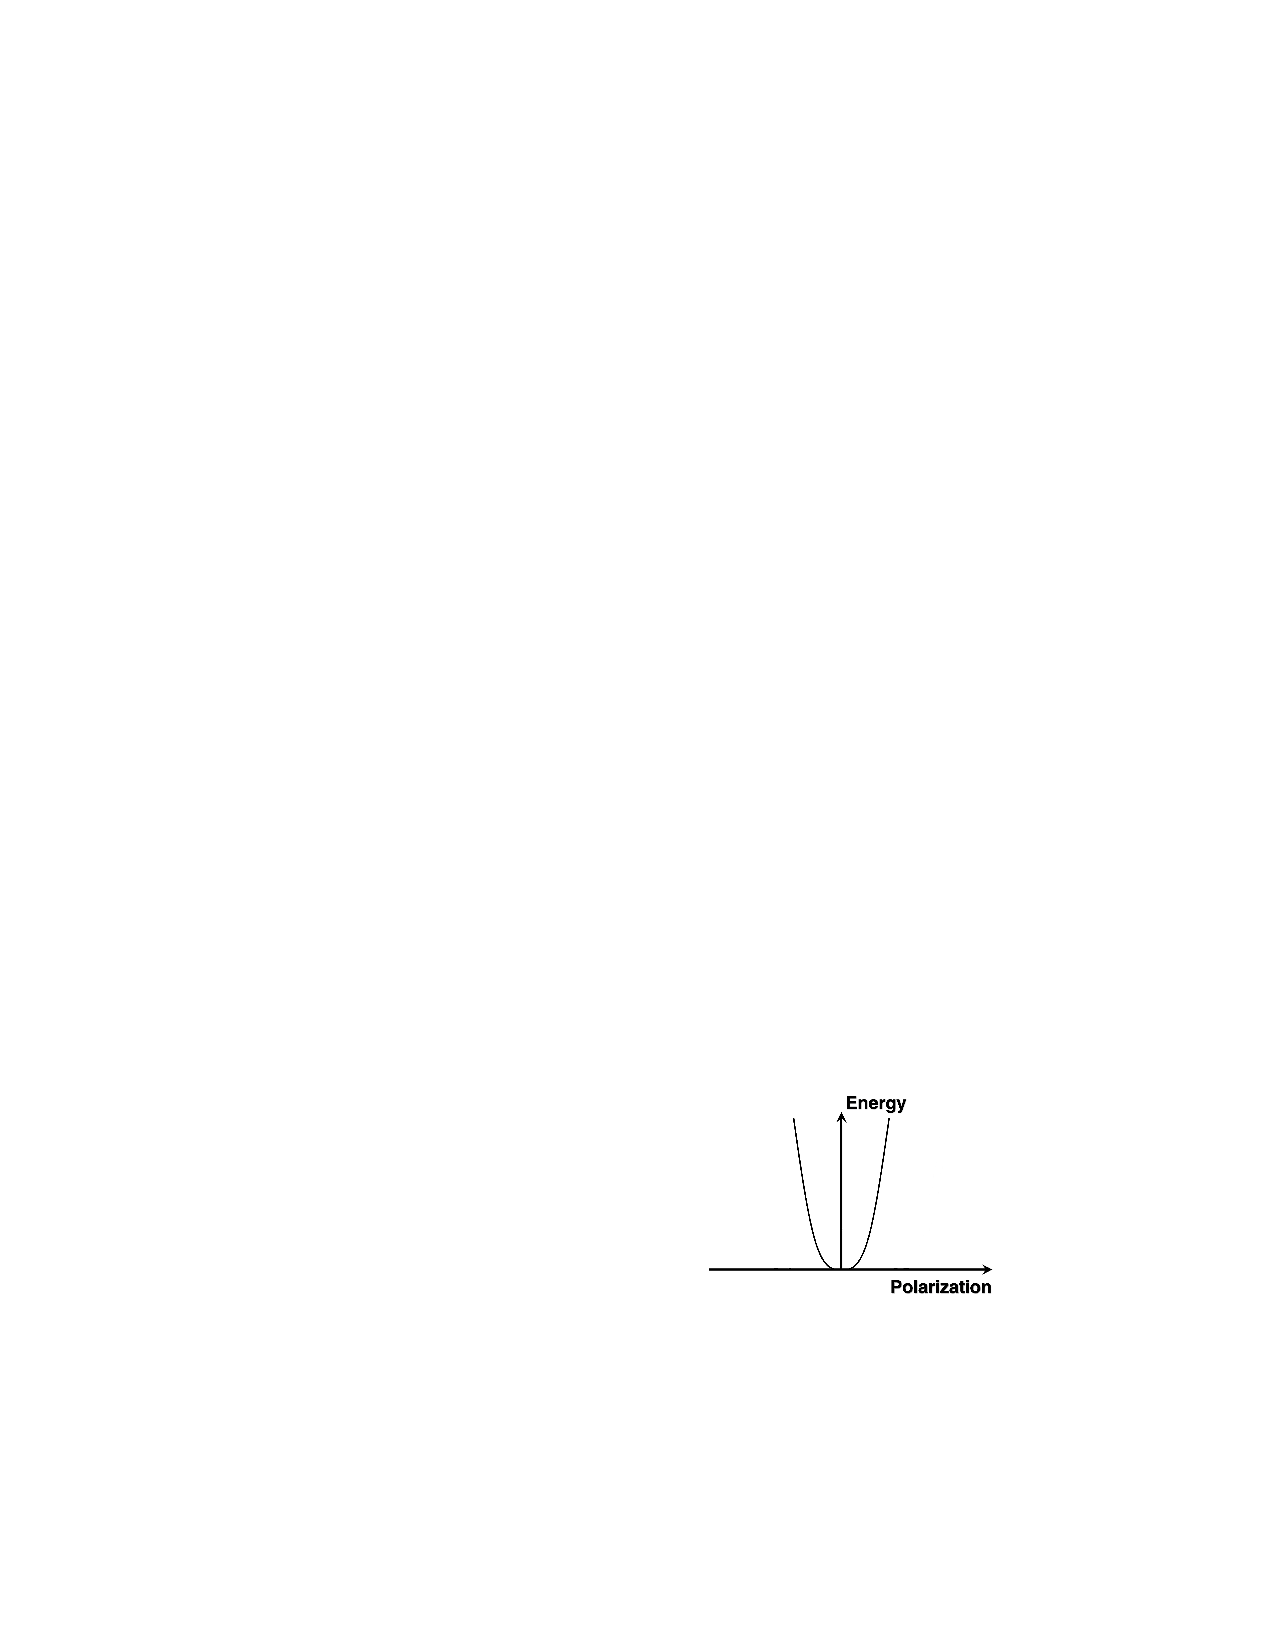
\includegraphics[width=0.45\linewidth]{./figures/materials/EvP-FE2}%
	} 	
   \subfloat[][Ferroelectric]{%
   	\label{fig:EvP-FE}%
	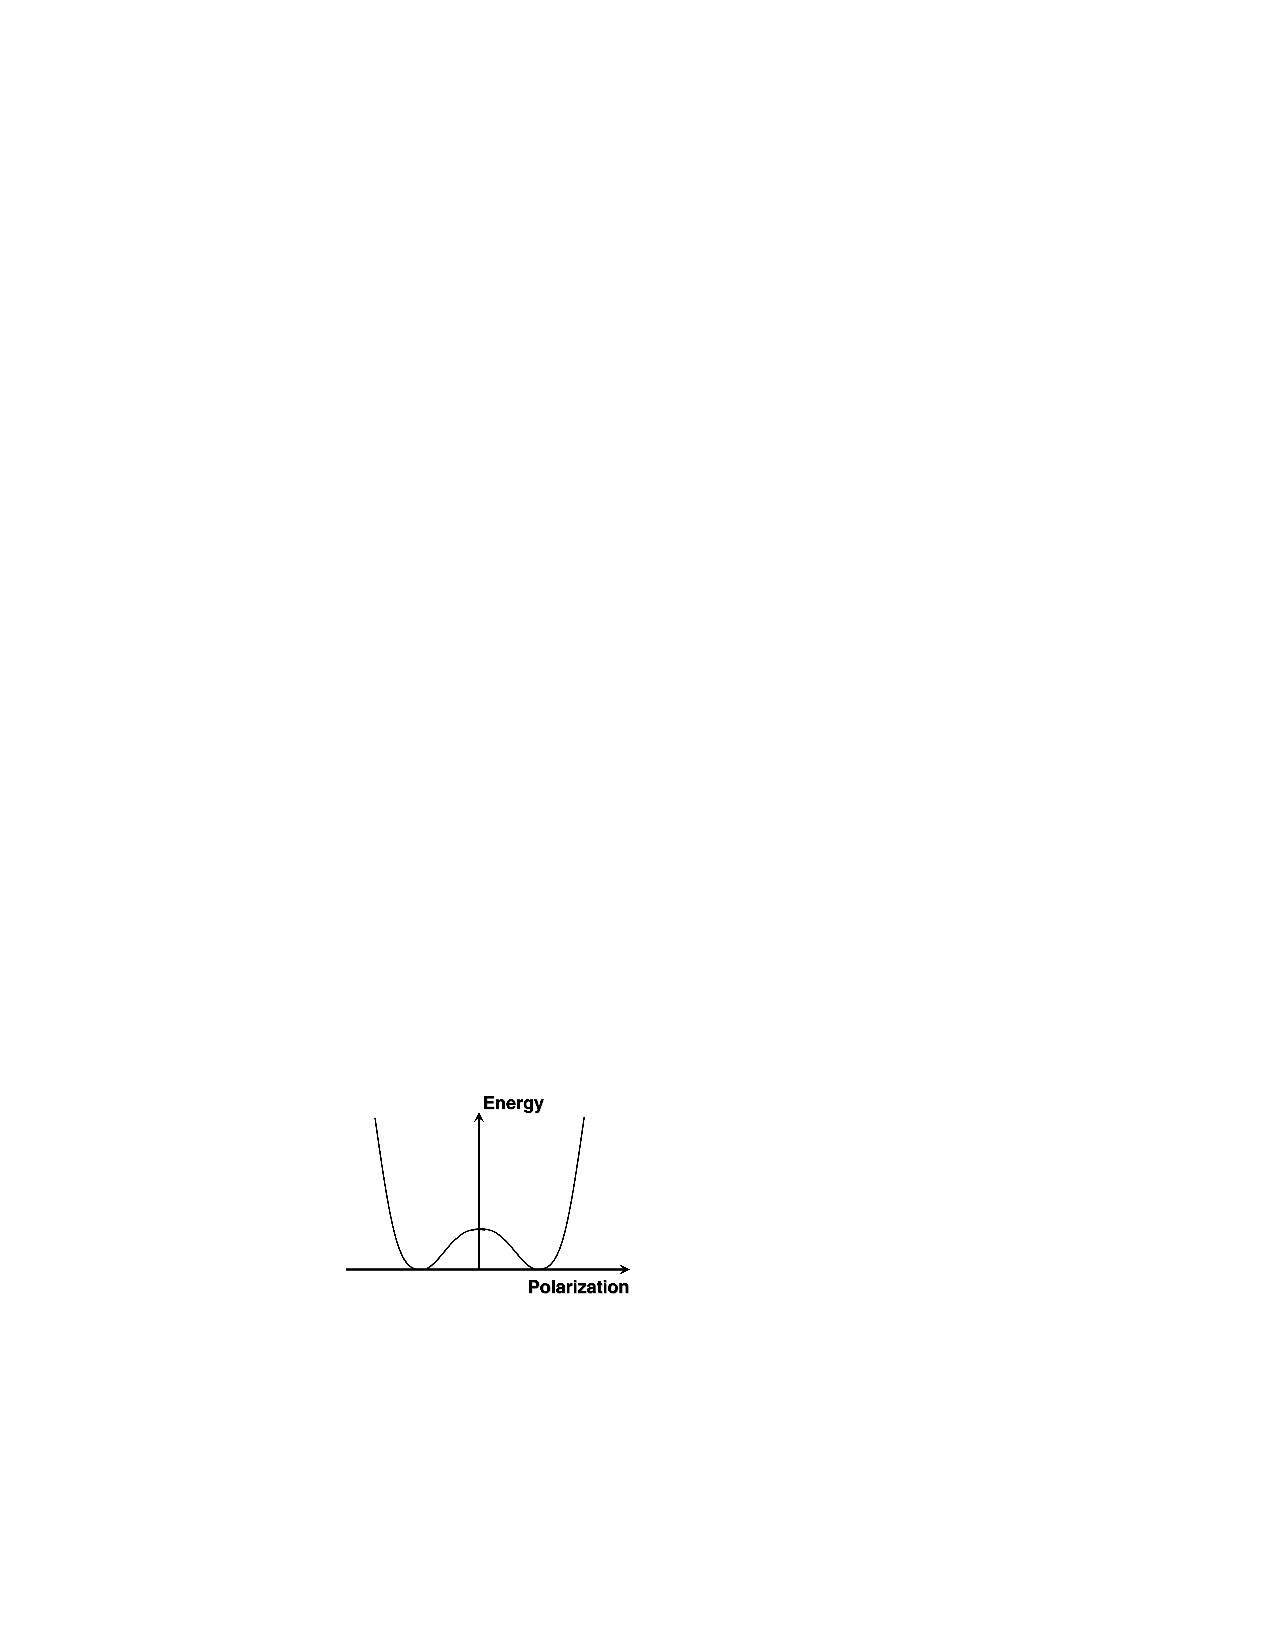
\includegraphics[width=0.45\linewidth]{./figures/materials/EvP-FE1}%
	} 	
   \caption[Energy vs. Polarization Plots for FE and PE Materials]%
   		{Example plots of the energy required to polarize a material. Ferroelectric materials (b) have %
		non-zero polarization at the energy minima. Above \Tc{} all ferroelectric materials transition %
		to a paraelectic phase (a). As temperature increases, the energy minima will approach one %
		another. }
   \label{fig:EvP}
\end{figure}

One of the most important effects of ferroelectric behavior is the exhibition of hysteresis in the polarization state of the material. \reword{Suboptimal explanations...} Because additional energy is required to make the transition from one state to another, the original state endures for some amount of opposing field (see fig.~\vref{fig:PvElec-FE}).

\begin{figure}[tb]
   \centering
   \subfloat[][Paraelectric]{%
   	\label{fig:PvElec-PE}%
	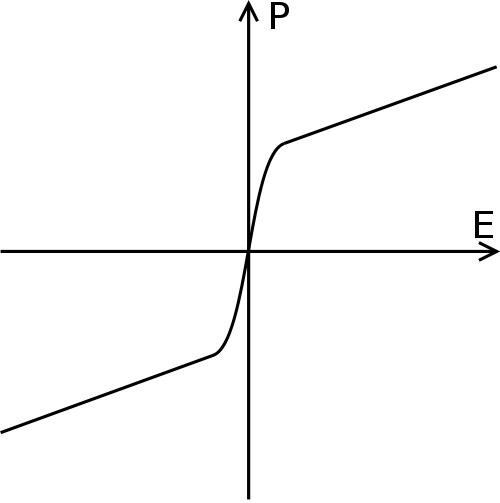
\includegraphics[width=0.4\linewidth]{./figures/materials/PvElec-PE}%
	} 
   \hspace{0.5cm}	
   \subfloat[][Ferroelectric]{%
   	\label{fig:PvElec-FE}%
	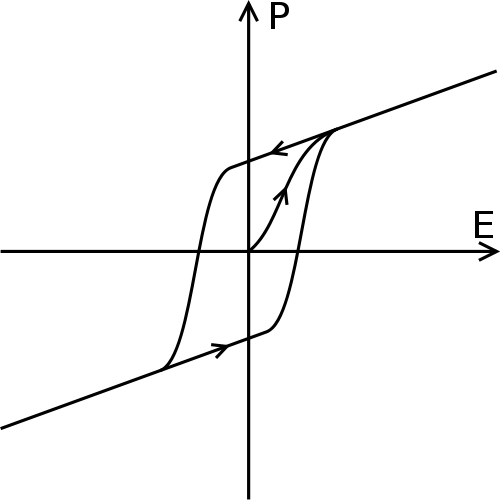
\includegraphics[width=0.4\linewidth]{./figures/materials/PvElec-FE}%
	} 	
   \caption[Polarization vs. Applied Field Plots for FE and PE Materials]%
   		{Example plots of the polarization as a function of applied field. (a) Paraelectric materials %
		have two regions of polarizability; at low E the polarization increases quickly with the field, %
		as E increases the rate of increase decreases. (b) Ferroelectric materials show similar %
		behavior, but additionally have hysteresis. This means that the films are switchable %
		between two states, but it is difficult to obtain zero polarization.}
   \label{fig:PvElec}
\end{figure}

%%%%%%%%%%%%%%%%%%%%%%%%%%%%%%%%%%%%%%%%%%%%%%%%%%%
%%%%%%%%%%%%%%%%%%%%%%%%%%%%%%%%%%%%%%%%%%%%%%%%%%%
%%%%%%%%%%%%%%%%%%%%%%%%%%%%%%%%%%%%%%%%%%%%%%%%%%%






























